% Generated by code/needham.py -- do not edit by hand.
\definecolor{qocA}{rgb}{0.00,0.45,0.70}
\definecolor{qocB}{rgb}{0.90,0.60,0.00}
\definecolor{qocC}{rgb}{0.00,0.62,0.45}
\definecolor{qocD}{rgb}{0.80,0.40,0.00}
\definecolor{qocE}{rgb}{0.80,0.60,0.70}
\definecolor{qocF}{rgb}{0.35,0.70,0.90}
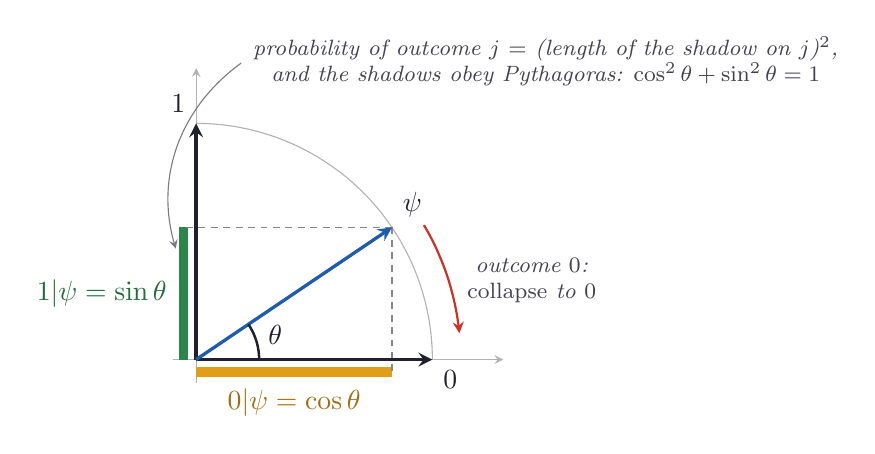
\begin{tikzpicture}[ink/.style={line width=0.9pt, ndInk}, faint/.style={line width=0.4pt, ndInk!35}, dashedink/.style={line width=0.5pt, ndInk!55, dash pattern=on 2.5pt off 2pt}, vec/.style={->, >=stealth, line width=1.2pt}, note/.style={font=\footnotesize\itshape, text=ndInk!85, align=center}, pointer/.style={->, >=stealth, line width=0.4pt, ndInk!60, shorten >=2pt, shorten <=1pt}, dot/.style={circle, fill=ndInk, inner sep=0pt, minimum size=3.4pt}, wash/.style={fill=ndSky, fill opacity=0.55}, every node/.style={text=ndInk}]
\definecolor{ndInk}{rgb}{0.13,0.13,0.18}
\definecolor{ndPaper}{rgb}{0.99,0.96,0.88}
\definecolor{ndSky}{rgb}{0.84,0.91,0.98}
\definecolor{ndRose}{rgb}{0.98,0.86,0.84}
\definecolor{ndBlue}{rgb}{0.13,0.36,0.66}
\definecolor{ndRed}{rgb}{0.78,0.20,0.16}
\definecolor{ndGold}{rgb}{0.88,0.62,0.10}
\definecolor{ndGreen}{rgb}{0.18,0.52,0.30}
\draw[faint] (3.000,0.000) -- (2.999,0.080) -- (2.996,0.160) -- (2.990,0.239) -- (2.983,0.319) -- (2.973,0.398) -- (2.962,0.477) -- (2.948,0.556) -- (2.932,0.634) -- (2.914,0.712) -- (2.894,0.789) -- (2.872,0.866) -- (2.848,0.942) -- (2.822,1.018) -- (2.794,1.092) -- (2.764,1.166) -- (2.732,1.240) -- (2.698,1.312) -- (2.662,1.383) -- (2.624,1.454) -- (2.585,1.523) -- (2.543,1.591) -- (2.500,1.658) -- (2.455,1.724) -- (2.408,1.789) -- (2.360,1.853) -- (2.310,1.915) -- (2.258,1.976) -- (2.204,2.035) -- (2.149,2.093) -- (2.093,2.149) -- (2.035,2.204) -- (1.976,2.258) -- (1.915,2.310) -- (1.853,2.360) -- (1.789,2.408) -- (1.724,2.455) -- (1.658,2.500) -- (1.591,2.543) -- (1.523,2.585) -- (1.454,2.624) -- (1.383,2.662) -- (1.312,2.698) -- (1.240,2.732) -- (1.166,2.764) -- (1.092,2.794) -- (1.018,2.822) -- (0.942,2.848) -- (0.866,2.872) -- (0.789,2.894) -- (0.712,2.914) -- (0.634,2.932) -- (0.556,2.948) -- (0.477,2.962) -- (0.398,2.973) -- (0.319,2.983) -- (0.239,2.990) -- (0.160,2.996) -- (0.080,2.999) -- (0.000,3.000);
\draw[faint, ->, >=stealth] (-0.3,0) -- (3.90,0);
\draw[faint, ->, >=stealth] (0,-0.3) -- (0,3.70);
\draw[line width=3.4pt, ndGold] (0,-0.160) -- (2.487,-0.160);
\draw[line width=3.4pt, ndGreen] (-0.160,0) -- (-0.160,1.678);
\draw[dashedink] (2.487,1.678) -- (2.487,-0.160);
\draw[dashedink] (2.487,1.678) -- (-0.160,1.678);
\draw[vec, ndInk] (0,0) -- (3.000,0) node[below right] {$\ket0$};
\draw[vec, ndInk] (0,0) -- (0,3.000) node[above left] {$\ket1$};
\draw[vec, ndBlue] (0,0) -- (2.487,1.678) node[above right] {$\ket\psi$};
\draw[ink] (0.800,0.000) -- (0.800,0.025) -- (0.798,0.050) -- (0.796,0.075) -- (0.794,0.100) -- (0.790,0.124) -- (0.786,0.149) -- (0.781,0.174) -- (0.775,0.198) -- (0.769,0.222) -- (0.761,0.246) -- (0.753,0.269) -- (0.744,0.293) -- (0.735,0.316) -- (0.725,0.339) -- (0.714,0.361) -- (0.702,0.383) -- (0.690,0.405) -- (0.677,0.426) -- (0.663,0.447);
\node at (1.004,0.307) {$\theta$};
\node[ndGold!70!black, below] at (1.244,-0.25) {$\braket{0|\psi}=\cos\theta$};
\node[ndGreen!80!black, left] at (-0.25,0.839) {$\braket{1|\psi}=\sin\theta$};
\draw[->, >=stealth, line width=0.8pt, ndRed] (2.893,1.708) -- (2.918,1.665) -- (2.943,1.621) -- (2.967,1.577) -- (2.990,1.533) -- (3.013,1.488) -- (3.035,1.443) -- (3.056,1.397) -- (3.076,1.351) -- (3.096,1.305) -- (3.115,1.259) -- (3.134,1.212) -- (3.152,1.165) -- (3.169,1.118) -- (3.185,1.070) -- (3.201,1.023) -- (3.216,0.975) -- (3.230,0.926) -- (3.243,0.878) -- (3.256,0.829) -- (3.268,0.781) -- (3.279,0.732) -- (3.290,0.683) -- (3.300,0.633) -- (3.309,0.584) -- (3.317,0.535) -- (3.325,0.485) -- (3.332,0.435) -- (3.338,0.385) -- (3.343,0.335);
\node[note, right] at (3.321,1.000) {outcome $0$:\\ \emph{collapse} to $\ket0$};
\node[note, anchor=south west] (m) at (0.6,3.35) {probability of outcome $j$ $=$ (length of the shadow on $\ket j$)$^2$,\\and the shadows obey Pythagoras: $\cos^2\theta+\sin^2\theta=1$};
\draw[pointer] (m.west) to[bend right=35] (-0.240,1.342);
\end{tikzpicture}
